\begin{refsegment}
	\chapter{Contexte biologique et méthodologique}

    Ce chapitre présente les notions biologiques puis informatiques, utilisées comme fondement du travail de recherche effectué lors de cette thèse.
    
    
    \section{Le métabolisme et sa représentation informatique}
    \subsection{Généralités sur le métabolisme}
    
    Pour perpétuer son espèce, tout organisme vivant consomme de l'énergie pour produire de la biomasse et se répliquer. Pour cela, l'être vivant doit assimiler des composés présent dans son environnement. Ces composés chimiques permettent de produire l'énergie, nécessaire \change{Vision Génome Centré}{David Vallenet} à la survie mais surtout à la transmission du patrimoine génétique. Ainsi on désigne par métabolisme, l'ensemble des processus de synthèse et dégradation de composés chimiques, mis en œuvre par l'organisme. De fait, les processus comme la réplication de l'\acrfull{ADN}, la traduction d'un gène et autres \ldots~sont exclus.
    
    \note{Le mot métabolisme à évolué à travers l'histoire pour nous parvenir sous ça forme actuelle. En grec ancien on utilise "\greekFont{μεταβολή}" équivalent à metabolé désignant "transformation". Le mot métabole signifie "qui subit un changement". Il a été utilisé par la suite comme mot racine: métabol-ique, métabol-isme \ldots
    }
    
    Les organismes vivant opèrent une multitude de transformations chimiques. Ils forment de véritable usine de traitement biochimique. En effet, ils disposent d'une batterie de réaction biochimique, afin de traiter un grand nombre de composés, tant à l'intérieur qu'à l'extérieur de la cellule. Par exemple, certains composés, de par la nature de la membrane cellulaire \footnote{La membrane cellulaire constitue une barrière physique entre le milieu extérieur et intérieur de la cellule.}, doivent être transformé depuis l'extérieur de la cellule, afin d'assimiler le composé transformé. De ce fait, la matière présente dans l'environnement est utilisé pour constituer les briques nécessaires au vivant.
    
    Par conséquent, le métabolisme est essentiel à la vie, d'une part il fournit l'énergie nécessaire. Et d'autre part, il va produire les molécules de base indispensables à l'organisme, pour sa construction, sa défense et autres \ldots
    
    Bien qu'agissant à une échelle moléculaire, le métabolisme d'un groupe d'organisme peut impacter son environnement. Si bien que les conséquences peuvent être observées à l'échelle humaine voire dans certains cas à l'échelle de la planète (voir Figure~\cref{fig:bloom}). Un autre exemple est celui des espèces végétales. Ils absorbent du dioxyde de carbone et produisent de l'oxygène. Ainsi ils jouent un rôle important dans la concentration de ces composés dans l’atmosphère.
    
    
    \begin{shadedfigure}[H]
        \begin{subfigure}[b]{.5\textwidth}
            \centering
            \includegraphics[width=\textwidth]{img/bloom_gascogne.jpg}
            \caption{{\tiny Source: \url{http://seos-project.eu}}}
            \label{fig:bloom_gascogne}
        \end{subfigure}
        \hfill
        \begin{subfigure}[b]{.5\textwidth}
            \centering
            \includegraphics[width=\textwidth]{img/bloom_bretagne.jpg}
            \caption{{\tiny Source: \url{https://commons.wikimedia.org/}}}
            \label{fig:bloom_bretagne}
        \end{subfigure}
        \caption{Le métabolisme d'un groupe d'individu produit une quantité de pigment photosynthétiques suffisamment conséquente, qu'il en devient observable depuis l'espace. Deux évènements distincts sont représentés. Le premier a eu lieu au large de la Gascogne le 17 mai 2004 et le second au niveau de la Bretagne le 15 juin 2004.}
        \label{fig:bloom}
    \end{shadedfigure}
    
    \note{Lors de l'apparition des premières formes de vie, il y a 3,6 milliards d’années. L'atmosphère était faiblement pourvue en oxygène. Ces organismes anaérobiques était présent dans les océans. L'oxygène est toxique, leur métabolisme s'est adapté au dioxyde de carbone, présent abondamment à ce moment. Puis entre 3,5 à 3 milliards apparurent des cyanobactéries. Ce sont des bactéries capable de capter l'énergie du soleil. Elles sont "photosynthétiques". Leurs métabolismes possèdent la particularité d'oxyder les minéraux présents dans les océans. Ils produisent ainsi de l'oxygène. Avec le temps leur métabolisme a consommé tellement de minéraux que l'oxygène produits dans les océans s’est libéré dans l’atmosphère. Modifiant ainsi fortement sa composition. Cet évènement influença le cours de la vie. De sorte que des organismes s'adaptent à l'oxygène. Car l'oxygène devient alors une molécule courante. Certaine forme de vie évolua jusqu'à devenir aérobie. Avec cet évènement, la Terre a subi sa première pollution atmosphérique d'ampleur induit par des organismes vivant. (Lire: \citetitle{bengtson1994early} ) }
    

    \change{a reprendre car tu mélanges les concepts}{David Vallenet}
    \change{Plus de contenu}{David Vallenet}
    
    \subsection{Les acteurs}
    
    L'étude du métabolisme est essentiel pour la compréhension des êtres vivants. Les débouchés impactent de nombreux domaines, tel que : la pharmaceutique, l'énergie, l'agriculture, l'environnement\ldots.  Pour mieux le comprendre, il est nécessaire d'introduire les différents acteurs du métabolisme. En effet, le métabolisme représente un ensemble d'événement faisant intervenir des métabolites, des réactions, des cofacteurs, des enzymes\ldots.
    
    
    
    \subsubsection{Les métabolites}
    
    Ce sont des composés organiques, de petites tailles, produits à travers les différents processus issus du métabolisme. Ils sont tour à tour synthétisés puis dégradés. Selon leurs rôles, ils interviennent soit dans les processus indispensables au développement et à la reproduction, dit "métabolisme primaire" . Soit pour des fonctions, non vitale comme la production d'antibiotique, de phéromone, de pigment \ldots, dénommé "métabolisme secondaire" .
    
    \note{Un composé organique s'oppose à un composé minéral. Cette différenciation s'explique par des raisons philosophiques antérieur au \siecle{19}. En effet, on distinguait les substances constitutives des organismes des autres. Ne sachant pas synthétiser les molécules organiques. On expliquait que l'intervention d'une "force vitale" était nécessaire. En 1828, Friedrich Wöler mis au point, accidentellement une expérience, produisant de l'urée (considéré comme organique) à partir de composé minéraux, comme le cyanate d’ammonium. Depuis lors, la notion de composé organique a évolué afin de désigner une molécule constituée d'une partie de carbone, le reste pouvant être des atomes d'hydrogène, oxygène azote et autres \ldots. La notion organique est resté car le carbone est un élément essentiel du vivant. Par opposition un composé minéral correspond à toutes molécules constituées d'élément autre que le carbone. Pour plus d'information, je vous invite à lire \citetitle{chimie_organique}.
    }    
      
    \change{ne pas mélanger le concept et enzymes}{David Vallenet}

	\subsubsection{Les réactions}
	Le processus de transformation d’un métabolite est décrit par une réaction. On désigne par le terme "substrat", les métabolites avant transformation. Par opposition, on parle de produit pour la molécule transformée. Ainsi une réaction est l'événement qui va transformer un substrat afin de produire un nouveau métabolite. Ces réactions s'effectuent au sein de l'organisme, dans l'infiniment petit, au niveau moléculaire.
    
    Une réaction est généralement représentée, par l’addition des molécules nécessaires à la transformation d’un côté. Puis de l’autre côté on expose la somme des molécules produites (voir \cref{fig:reaction}). Cette équation  représente la stœchiométrie de la réaction. C’est-à-dire que la proportion des éléments en jeu avant et après la réaction est respectée. De tels réactions sont représentées à l'équilibre, c'est-à-dire que la proportion de chaque atome est identique entre avant et après la réaction. Pour reprendre la célèbre maxime "Rien ne se perd, rien ne se crée, tout se transforme" .
    
    \begin{shadedfigure}[H]
        \centering
        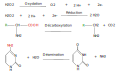
\includegraphics[width=\textwidth]{img/equation_reaction.pdf}
        \caption{Représentation de réaction sous leur forme "équation-bilan" .}
        \label{fig:reaction}
    \end{shadedfigure}
    
    \citation{ On voit que, pour arriver à la solution de ces deux questions, il fallait d'abord bien connaître l'analyse et la nature du corps susceptible de fermenter, et les produits de la fermentation ; car rien ne se crée, ni dans les opérations de l'art, ni dans celles de la nature, et l'on peut poser en principe que, dans toute opération, il y a une égale quantité de matière avant et après l'opération ; que la qualité et la quantité des principes est la même, et qu'il n'y a que des changements, des modifications }{Antoine Lavoisier}[Traité élémentaire de chimie, 1864]
    
    
    \subsubsection{Les enzymes}    
    La plupart de ces transformations ne sont pas spontanées où se feraient trop lentement. Pour cela, l'organisme dispose de molécule protéique facilitant ces transformations, appelé "enzyme". Ce sont des bio-catalyseurs, c'est-à-dire qu'elles vont favoriser ou accélérer une transformation chimique. Ces molécules peuvent couper, coller, réparer synthétiser ou encore modifier une molécule. Elles ont la particularité d'avoir une forte affinité avec leur substrat.  Leur rencontre provoque une transformation du composé. Puis, le ou les produits résultant de cette transformations, peuvent êtres à leur tour reconnu par d'autres enzymes. Provoquant ainsi une cascade de transformation chimique. 
    
    Une enzyme est une molécule constituée d'acide aminé, dont sa structure tri-dimensionnel contient des régions impliquées dans la reconnaissance et la transformation d’une molécule. C'est pourquoi, une même enzyme reconnaît une ou plusieurs molécules spécifiquement et induit les mêmes transformations chimiques. Ce processus est décrit par le modèle de "clef / serrure" (voir \cref{fig:reaction_enzymatique}). Le plus couramment les enzymes sont répertoriées selon quatre numéros séparé par des points désignant la réaction chimique qu'elles catalysent. C'est le système de nomenclature \acrfull{EC}. Chaque nombre est associé à un concept. Ainsi le premier indique le type de réaction catalysé,  le second décrit la catégorie du substrat utilisé, le troisième correspond au substrat spécifiquement impliqué et enfin le quatrième le numéro de série de l'enzyme.
    
    \begin{shadedfigure}[H]
        \centering
        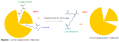
\includegraphics[width=\textwidth]{img/lysine-oxoglutarate_reductase.pdf}
        \caption{Schéma d'une réaction chimique catalysée par une enzyme. L'enzyme reconnaît ces substrats 2-oxoglutarate et L-Lysine, puis les transforme en une molécule de L-Saccharopine. La molécule NADPH$^{+}$ est nécessaire à l'activité enzymatique. On parle de cofacteur.}
        \label{fig:reaction_enzymatique}
    \end{shadedfigure}
    
    Une enzyme possède une affinité importante avec son substrat. Cette affinité influe sur l’activité enzymatique, c’est-à-dire sur la vitesse de transformation du substrat. Il existe des molécules, autres que les substrats de l’enzyme,  avec  une forte affinité pour l’enzyme. De tels molécules vont diminuer l’activité enzymatique. Les inhibiteurs enzymatiques joue un rôle important dans le métabolisme. Ils sont employés comme régulateurs du métabolisme. 
    
    \note{
        Les inhibiteurs enzymatiques permettent de limiter voir d’arrêter l’activité d’une enzyme. Cette caractéristique est employée pour  tuer des organismes pathogènes. Par exemple, La Pénicilline est un inhibiteur de la  transpeptidase intervenant dans la synthèse du peptidoglycane. Le peptidoglycane forme la paroi des bactéries. Si cette dernière est dans l’incapacité de synthétiser ça paroi alors cela conduit à la mort de la bactérie.
    }

    \subsubsection{Les cofacteurs}
    Certaines réactions nécessitent l’apport d'énergie, d’ion ou encore de molécules d'assistance qui vont favoriser l’activité enzymatique. \textbf{(trop brut pas de liaison)} Les enzymes nécessitant l'apport de cofacteur sont appelées holoenzyme lorsque le cofacteur est liée à cette dernière. Par opposition une enzyme inactive non lié à son cofacteur est une apoenzyme. Les cofacteurs sont classifiés en deux catégories : les ions métalliques et les coenzymes.
    
    Les ions métalliques de par leurs charges positives permettent de contre-balancer les charges négatives, amener soit par les chaines d'histidines de l'enzyme soit lors de la réaction catalytique \cite{christianson1991structural}. Dans le premier cas l'ion métallique joue un rôle structural au sein de l'enzyme. Dans le second il va assister l'enzyme dans son processus de transformation tout en maintenant sa structure. Effectivement les ions métalliques de part leur nature peuvent assister l'enzyme lors des réactions d'oxydoréduction et de transfert d'électron. Les ions fréquemment observé dans le vivant sont les ions fers, cuivres, zincs et magnésiums.
    
    Les coenzymes sont des molécules organiques. Elles sont rangées en deux groupes en fonction de la nature de la liaison établie avec l'apoenzyme.
    
    Le premier groupe contient les cofacteurs liés faiblement à l'enzyme. Ces cofacteurs subissent généralement une transformation lors de la réaction. Pour cette raison ils sont également appelé co-substrat. Par exemple une des réactions de la glycolyse implique le cofacteur NADP$^{+}$ pour transformer le glucose-6-phosphate (voir \cref{eq:glucose}). Ce cofacteur  se lie à l'enzyme puis il est transformé au cours de la réaction en NADPH. Cette modification engendre la libération du cofacteur de l'enzyme. Ce groupe contient également des cofacteurs énergétiques, c'est-à-dire que la transformation du cofacteur va engendrer une libération d'énergie. Cette énergie permet de réaliser des transformations qui était dans la cellule énergétiquement défavorable. De nombreux mécanismes essentiels au vivant nécessite l'apport d'énergie. Pour ces raisons le métabolisme d'un organisme est adapté à son environnement afin de produire l'énergie indispensable à sa survie et sa reproduction. Majoritairement le nucléotide \acrfull{ATP} est utilisé par le vivant comme cofacteur énergétique. L'hydrolyse de l'\acrfull{ATP} en \acrfull{ADP} induit la coupure d'une liaison avec un phosphate provoquant une libération d'énergie. On retrouve également d'autres cofacteurs utilisant la guanine, la thymine, la cytosine ou encore l'uracile en lieu et place de l'adénine (respectivement  GTP, TTP, CTP et UTP ). Le vivant est en perpétuel déséquilibre énergétique de part les différents processus qui le constitue, l'apport énergétique permet le maintien de la vie.
    
    \begin{equation}\label{eq:glucose}
        glucose-6-phosphate + NADP^{+} \rightarrow 6-phosphoglucono-D-lactone + NADPH + H^{+}
        \stepcounter{equation}\tag{équation \theequation}
    \end{equation}
    
    Le deuxième groupe de coenzyme représente les cofacteurs liés de façon covalente \footnote{Une liaison covalente est une liaison chimique dans laquelle deux atomes sont mutuellement attirer par une force. Cette force provient de la mise en commun d'au moins un électron par atome.} à l'enzyme. Ils sont appelés "groupements prosthétiques". Un des exemples les plus connu et celui de l'hème des hématies. C'est un groupement contenant un atome de métal (souvent le fer) permettant de capturer un gaz diatomique comme le dioxygène (O${2}$) où encore le monoxyde de carbone (CO).
    
    Ainsi le vivant via ces différents acteurs possèdent des combinaisons de réactions lui procurant les moyens de vivre et de se reproduire. Ces successions de réactions sont humainement représentées selon des objectifs considérés d'intérêts biologiques. Pour cette raison un cheminement de transformation métabolique en métabolique est appelé "voie métabolique".
    
    
    \subsubsection{Voies métaboliques}
    On distingue dans le métabolisme deux catégories de processus, l'anabolisme et le catabolisme. L'anabolisme, représente l'ensemble des réactions impliqué dans la synthèse de nouvelle molécule. La production de nouveaux composés nécessite de l'énergie. De tels processus sont constitués de réaction endergonique. Ainsi le bilan énergétique est négatif.  Au contraire, le catabolisme décrit l'ensemble des réactions de dégradation de molécule. Les réactions impliquées dans la dégradation d'une composé, produisent in-fine plus d'énergie qu'elles en on consommé. Ces réactions produisant de l'énergie sont dites exergoniques.
    
    Ces notions permettent de diviser l'ensemble des processus du métabolisme en sous-parties plus faciles à appréhender. Toujours dans l'intention de réduire l'énorme quantité de concept. Les réactions sont regroupées dans différentes entités appelées "voie métabolique". Ce découpage permet de représenter des segments d'évènement de transformation métabolique en ensemble de réaction permettant de réaliser un objectif d'intérêt biologique. Certains objectifs peuvent être atteints par des successions de réactions différentes. Ainsi une même voie métabolique peut être réalisé par différents chemins de réaction.
    
    Étant donnée que ces modules métaboliques réalise des transformations apportant un avantage à la cellule. Ces modules via le principe de pression de sélection vont tendre à garder la même structuration \cite{braakman2012compositional}. Les gènes correspondant aux protéines impliquées dans ces voies sont souvent co-localisées sur le génome. En effet une telle disposition des gènes favorise l'expression de toutes les protéines nécessaires pour la réalisation de l'objectif biologique à un instant "\textit{t}". De tels dispositions simplifie le processus de régulation d'expressions de ces gènes. Ce qui se traduit souvent par un gain énergétique donc un avantage évolutif pour la cellule. Comprendre la structuration du métabolisme, c'est également expliquer comment la physique et la chimie ont contraint la vie et l'évolution.
    
    Ces voies métaboliques sont des réactions connectées les unes aux autres. Ils se représentent intuitivement sous forme de graphe.
    
    \subsection{Représentation en graphe}
    
    De tels représentations permettent de partager des notions complexes sur un grand nombre de concepts ainsi que leurs relations. Les graphes s'avèrent utile pour l'étude des divers réseaux. Par exemple, le réseau routier, ça représentation est intuitive et permet la mise œuvre d'algorithme de recherche du plus court chemin. Cette branche des mathématiques s'est illustrer à travers la résolution  de problème complexe comme la traversée des sept ponts de Königsberg, la marche du cavalier sur l’échiquier et bien d'autres. Les applications des recherches issue de la théorie des graphes sont multiples. On retrouve son utilisation dans des domaines comme la chimie, le stockage de donnée (à travers les bases de données type graphe), l'ontologie (et ces relations entre les concepts), la biologie et ces différents réseaux (dont le métabolisme). Cette représentation de l'information à montrer son utilité à des problèmes complexe très variés.
    
    Avant d'aller plus loin, il est nécessaire de définir plusieurs notions employées dans la théorie des graphes. Tout d'abord un graphe est constitué de nœud relié entre eux. Les nœuds du graphe sont également appelés sommets ("vertice" en anglais).  Lorsque les relations indique un sens de cheminement entre deux nœuds ("edge" en anglais), elles sont qualifiés d'arc autrement on parle d'arrête. Ainsi on fait la distinction en graphe orienté et non-orienté. Généralement un graphe est désigné sous la forme mathématique :
    
    \begin{equation}\label{eq:graph}
    	G = (V,E) \stepcounter{equation}\tag{équation \theequation}
    \end{equation}
    
    Dans l'\cref{eq:graph}, G désigne le graphe tel que constitué de deux ensembles, celui des sommets V et celui des relations V. Différents type de graphe sont présentés dans la \cref{fig:graphe}.
    
    
    \begin{shadedfigure}[H]
    	\centering
    	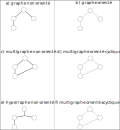
\includegraphics[width=\textwidth]{img/graph.pdf}
    	\caption{a) un graphe  avec des arrêtes. b) Un graphe avec des arcs indiquant une orientation entre deux sommets. c) un multigraphe non orienté avec des arêtes reliant les deux mêmes sommets. d) un multigraphe dont les relations forme un chemin cyclique à travers les sommets. e) un graphe avec une hyperarête reliant deux sommets. f) un multigraphe avec une orientation des relations tels que le chemin à travers le graphe traverse qu'une seule fois les sommets. }
    	\label{fig:graphe}
    \end{shadedfigure}
    
    
    
    Dans le cadre de la biologie, de nombreux évènements se représentent sous forme de réseaux. Pour en citer quelques uns, il y a les réseaux : d'interactions physiques protéine-protéine, de régulation de l'expression des gènes, de maximisation de flux (\acrfull{FBA}), de réaction métabolique… 
    
    Dans ce chapitre allons nous intéresser à la représentation en graphe des voie métaboliques. 
    
    \subsection{Ressources sur les voies métaboliques}
    
    Une voie métabolique est un enchainement de réaction enzymatique durant lequel les métabolites sont transformés. Ils représentent usuellement une fonction biologique. Par conséquent ces fonctions sont susceptibles d'être partagés à travers le monde du vivant. Toutefois pour réaliser une fonction biologique, il peut exister plusieurs variantes de chemin réactionnel. Par exemple pour la biosynthèse de la L-lysine, six voies alternatives sont connus à ce jour dans le monde du vivant (voir \cref{fig:lysine} ).
    	
    	
    	\begin{shadedfigure}[H]
    		\centering
    		\includegraphics[width=\textwidth]{img/L-lysine-biosynthesis.jpg}
    		\caption{Biosynthèse de la L-Lysine peut se faire par via la voie DAP et ses quatre chemins de réactions possibles où via la voie AAA et ces deux voies alternatives. Figure reprise de l'article \citetitle{morgat2011unipathway}. }
    		\label{fig:lysine}
    	\end{shadedfigure}
     
     La représentation des voies métaboliques est une synthèse d'évènements se produisant dans le vivant. Par conséquent cette représentation est subjective. Elle diffère selon les éléments souhaitais être en avant où bien encore selon les informations et les meta-informations dont dispose la ressource. Ces différences seront exposées à travers les ressources sur les voies métaboliques KEGG, Reactome, Unipathway, Genome properties.
     
    \subsubsection{KEGG}
    
    La ressource \textit{KEGG} (pour "Kyoto Encyclopedia of genes and Genomes") \cite{ogata1999kegg,kanehisa2000kegg,kanehisa2002kegg,kanehisa2004kegg,aoki2005using,kanehisa2010kegg,kanehisa2017kegg} est une ressource de données pour comprendre les fonctions globales et les utilités du système biologique, telles que la cellule, l'organisme et l'écosystème. Pour cela \textit{KEGG} dispose d'un point d'entré principale \url{http://www.genome.jp/kegg/kegg2.html}. Ce point d'entrée liste les trois orientations proposé par \textit{KEGG}.
    
    La première entrée est "orienté donnée", elle comprend les informations relatives à: la biologies des systèmes\footnote{Domaine d'étude pour la compréhension des interactions entre les différentes parties du système biologique, tels que les réseaux de gènes et de protéines, les organites et autres \ldots. } , génomiques, chimiques et de santé (voir le détail dans le \cref{tab:kegg_data_oriented}). Le second point d'entrée dit "sujet orienté" propose des informations relatives à une thématique comme le cancer (\textit{KEGG Cancer}), les pathogènes (\textit{KEGG Pathogen}), les virus (\textit{KEGG virus}) et autres \ldots. Le dernier point d'entrée corresponds aux informations spécifiques à un organisme via \textit{KEGG organism}. Ce catalogue contient les génomes complétement séquencés de 346 eucaryotes, 4039 bactéries et 243 archées.  
    
    
    \begin{table}[H]
        \small
        \caption{Détail du point d'entrée "orienté donnée". }\label{tab:kegg_data_oriented}
        \label{tab:kegg_oriented_data} 
        \begin{tabular}{p{0.2\linewidth}|p{0.3\linewidth}|p{0.5\linewidth}}
            \toprule
            Catégorie               & Point d'entrée                                                        & Contenu \\
            \midrule
            Biologie des systèmes  & \href{http://www.genome.jp/kegg/pathway.html}{KEGG PATHWAY}           & Carte métabolique \\   
            \cline{2-3}
                                    & \href{http://www.genome.jp/kegg/brite.html}{KEGG BRITE}               & Structuration hiérarchique de fonction biologique \\
            \cline{2-3}             & \href{http://www.genome.jp/kegg/module.html}{KEGG MODULE}             & Collection d'unité fonctionnelle utilisé pour l'annotation génomique et l'interprétation biologique \\
            \hline
            Génomique               & \href{http://www.genome.jp/kegg/genome.html}{KEGG GENOME}             & Collection d'organisme \textit{KEGG} complétement séquencé. \\
            \cline{2-3}             & \href{http://www.genome.jp/kegg/genes.html}{KEGG GENES}               & Catalogue de gènes et protéines \\
            \cline{2-3}             & \href{http://www.kegg.jp/kegg/ssdb/}{KEGG SSDB}                       & Base de donnée sur la similarité des séquences d'acide aminé à partir de tous les gènes codant pour des protéines dont le séquençage et complet \\
            \cline{2-3}             & \href{http://www.genome.jp/kegg/ko.html}{KO (KEGG Orthology)}         & Association des fonctions biologiques aux différents groupes orthologues  \\
            \hline
            Chimie                  & \href{http://www.genome.jp/kegg/compound/}{KEGG COMPOUND}             & Ensemble de petite molécule d'intérêt biologique\\
            \cline{2-3}             & \href{http://www.genome.jp/kegg/glycan/}{KEGG GLYCAN}                 & Collection de structure de glycane expérimentalement observé \\
            \cline{2-3}             & \href{http://www.genome.jp/kegg/reaction/}{KEGG REACTION}             & Banque de donnée répertoriant les réactions chimiques dont les réactions enzymatiques\\
            \cline{2-3}             & \href{http://www.genome.jp/kegg/annotation/enzyme.html}{KEGG ENZYME}  & Catalogue d'enzymes associé à leurs numéros \acrfull{EC}\\
            \hline
            Santé                   & \href{http://www.genome.jp/kegg/disease/}{KEGG DISEASE}               & Fournit des cartes représentant les différents perturbateurs. Ces perturbateurs peuvent être géniques, infectieux, multi-factorielle \ldots\\
            \cline{2-3}             & \href{http://www.genome.jp/kegg/drug/}{KEGG DRUG}                     & Classification et description des drogues autorisées au Japon, USA et en Europe\\
            \cline{2-3}             & \href{http://www.genome.jp/kegg/drug/environ.html}{KEGG ENVIRON}      & Est une collection de médicaments, d'huiles essentielles et d'autres substances favorisant la santé, qui sont pour la plupart des produits naturels de plantes \ldots Cette base complète la ressource \textit{KEGG DRUG}.\\
            \cline{2-3}             & \href{http://www.genome.jp/kegg/medicus.html}{KEGG MEDICUS}           & Est une ressource faisant la synthèse des autres  bases orienté-santé \\
            \bottomrule
        \end{tabular}
    \end{table}
    
    
    Les différents acteurs du métabolisme sont répartit à travers les bases de données \textit{KEGG LIGAND} pour les métabolites, \textit{KEGG REACTIONS} pour les réactions et \textit{KEGG ENZYME} pour les enzymes.
    
    En ce qui concerne la représentation du métabolisme, \textit{KEGG PATHWAY} organise le réseau métabolique en un graphe dirigé (voir \cref{fig:kegg_lysine}). Ce réseau est découpé sous forme de carte répertoriant toutes les réactions supposées avoir lieu dans le domaine du vivant. La construction de ce réseau provient essentiellement de prédiction bio-informatique.
    
    \begin{shadedfigure}[H]
        \centering
        \includegraphics[width=\textwidth]{img/kegg_lysine.png}
        \caption{ Représentation du réseau métabolique selon un graphe dirigé. Les sommets du graphe sont des métabolites et les arcs correspondent aux réactions. Carte extraite de la ressource en ligne "KEGG pathway". }
        \label{fig:kegg_lysine}
    \end{shadedfigure}
    
    \subsubsection{Reactome}
    Le projet Reactome \cite{joshi2005reactome,matthews2009reactome,croft2010reactome,croft2014reactome,fabregat2016reactome} met à la disposition de la communauté des voies métaboliques expertisées et vérifiées par l'Homme. Différentes vues sont proposées selon le niveau hiérarchique du concept sélectionné (voir \cref{fig:reactome_metabolism} et \cref{fig:reactome_serine}). Cette ressource contient à ce jour 19 organismes eucaryotes. La curation puis l'organisation des données est couteuse en temps. Pour ce donner un ordre d'idée sur l'avancement du travail d'expertise et d'intégration la version 54 de septembre 2015 comprenait 43\% des gènes humains. Ceci représente un total de 8701 gènes sur les 20 296 gènes codant pour des protéines prédits.
    
    \begin{shadedfigure}[H]
        \begin{subfigure}[t]{.5\textwidth}
            \centering
            \includegraphics[angle=90,origin=c,width=\textwidth]{img/reactome_homo_sapiens_metabolism.png}
            \caption{ Vue globale des relations ontologique chez l'Homme sous forme de graphe hiérarchique. En naviguant du centre vers l'extrémité des sous-graphes, les concepts vont des plus généraux aux plus spécifiques. }
            \label{fig:reactome_metabolism}
        \end{subfigure}
    \hfill
    \begin{subfigure}[t]{.45\textwidth}
        \centering
        \includegraphics[width=\textwidth]{img/reactome_homo_sapiens_serine_biosynthesis.png}
        \caption{ Représentation du réseau métabolique selon un hypergraphe dirigé. Les sommets verts sont les métabolites et cofacteur participants à la réaction. Les réactions correspondent aux sommets représenté par des carrés blancs. Les sommets cerclés de bleu sont les étiquettes attachées à la réaction, afin d'indiquer le nom de l'enzyme, le numéro \acrfull{EC} de la réaction et autres informations\ldots. Les hyperarêtes indique le sens de la réaction et pointes sur les molécules transformées. }
        \label{fig:reactome_serine}
    \end{subfigure}
    \end{shadedfigure}

    \subsubsection{Unipathway}
    
    Cette ressource en ligne fournissait un travail de curation des voies métaboliques \cite{morgat2011unipathway}. C'est-à-dire qu'il y avait une validation des voies métaboliques prédites par de l'expérimentation et/ou de l'expertise humaine. Le réseau métabolique est découpé en cinq concepts, les voies métaboliques (\acrfull{UPA}), les chemins réactionnels linéaires (\acrfull{ULS}), les réactions enzymatiques (\acrfull{UER}), les réactions chimiques (\acrfull{UCR}) , les composés (\acrfull{UPC}) (voir \cref{fig:unipathway_structure}). Ces concepts sont ordonnés les uns par rapport aux autres via des relations de compositions et d'équivalence. Le modèle est très flexible il fait une distinction entre réaction chimique et réaction enzymatique. En effet une réaction chimique peut être spontané et/ou être réalisé par différent bio-catalyseur. Enfin à travers le concept d'\acrfull{ULS}, la ressource fait apparaître les enchainements de réactions permettant de réaliser un objectif biologique. Un \acrfull{ULS} est un ensemble réaction (\acrfull{UER}) impliqué dans une seule tâche biologique. Ainsi les \acrfull{ULS} comprenant plusieurs réactions, sont délimités par des réactions impliquée dans au moins deux processus biologiques. Cependant, il est très fréquent de voir une même réaction impliquée dans plusieurs processus biologiques. C'est pourquoi seulement 30\% des \acrfull{ULS} ont plus de deux réactions. Toutefois un incident technique a provoqué l'arrêt de ce projet. Cette base d'information est encore à ce jour indisponible : \url{http://www.unipathway.org/}.
    
    \note{
    	Selon le fournisseur d'internet néozélandais "\textit{Actrix}":
    	\begin{itemize}
    		\item 60\% des compagnies ayant perdu toutes leurs données ont fermé dans les 6 mois après l'évènement.
    		\item Il est estimé pour une heure de travail les données perdues coûte en moyenne à une entreprise 790 \$.
    		\item 31\% de la perte de donnée de plus de 500 000 \$ est due à une défaillance du système.
    		\item Un disque dur sur cinq est bloqué au cours de sa vie.
    	\end{itemize}
    	{\tiny Source: \url{http://editor.actrix.co.nz/0305.htm}.}
    }
    
    
    \begin{shadedfigure}[H]
        \centering
        \includegraphics[width=\textwidth]{img/unipathway_structure.jpeg}
        \caption{ Overview of the UniPathway concepts. (a) Unified Modeling Language (UML)-like representation of the UniPathway classes and relationships. Legend is to the right of the main part of the figure. Multiplicity constraints read as: One UPA is composed of 0 or more ULS—One ULS is contained in exactly 1 UPA. One ULS is composed of 1 or more UER—One UER is contained in exactly 1 ULS. One UER is composed of 0 or more (alternate) UER—One UER is contained in 0 or at most 1 UER. One UER is composed of 0 or more UCR—One UCR is contained in 1 or more UER. One UCR is composed of 1 or more left UPC and 1 or more right UPC—One UPC is contained in 1 or more UCR. (b) Example of the IsA relationship defining the UniPathway controlled vocabulary hierarchy of pathway terms. A pathway instance may be a specific type of an abstract pathway entity. (c) Example of the PartOf relationship linking a pathway (UPA: light blue), its subpathways (ULS: blue) and individual enzymatic reactions that constitute the subpathway (UER: dark blue). (d) Three cases of the relationship between an UER and its chemical reaction components (UCR): (1) simple one-to-one relationship where R is catalyzed by a single enzyme; (2) R is catalyzed by an enzyme and S is a spontaneous reaction; (3) ‘OR’ relationship: the enzyme can catalyze two reactions differing by their co-substrates (e.g. NADH/NADPH).}
        \label{fig:unipathway_structure}
    \end{shadedfigure}

    \subsubsection{BioCyc et MetaCyc}
    
    \textit{BioCyc} \cite{caspi2006metacyc,caspi2007metacyc,caspi2008metacyc,caspi2010metacyc,caspi2012metacyc,caspi2013metacyc,caspi2014metacyc,caspi2015metacyc,caspi2016metacyc} est une collection en ligne (\url{https://biocyc.org/}) de voie métabolique et de génome (dénoté PGDBs pour "Pathway/Genome DataBases"). Cette resource fournit des données de qualtité à travers une sructure multi-couche afin d'avoir un panel d'information large et cohérent (voir \cref{fig:biocyc_collection}) . Ajouté a ces données biologiques, BioCyc fournit des outils pour leurs explorations et compréhensions. Les PGDBs \textit{BioCyc} sont générées par un logiciel de prédiction des voies métaboliques nommé "PathwayTools" \cite{karpe2011pathway,karp2015pathway}. De plus il identifie les opérons \cite{romero2004using} et suggère des gènes pour les enzymes orphelines\footnote{Une enzyme est dites orpheline lorsque l'on n'est pas capable de l'associé à un gène.}\cite{Green2004}. \textit{BioCyc} intègre également les informations d'autres bases de données de bioinformatics, telles que les caractéristiques des protéines et l'information ontologique d'\textit{UniProt} portant sur les gènes . Le site Web \textit{BioCyc} offre une suite d'outils logiciels pour la recherche, l'analyse et la visualisation de donnée métabolique.
    
    
    \begin{shadedfigure}[H]
    	\centering
    	\includegraphics[width=\textwidth]{img/BioCycCollection.png}
    	\caption{\textit{BioCyc} est un ensemble de base de donnée et d'outil sur le métabolisme. \textit{Metacyc} regroupe l'ensemble des informations du monde vivant. Cette ressource comprend 2255 voies métaboliques à ce jour. Ces données biologiques sont répartis à travers 3 couches (i.e "Tiers"). Ces couches classifient le niveau de qualité des bases de données  (Du moins vers le plus qualitatif : tiers 3 à 1). \hspace{\textwidth} Source : \url{https://biocyc.org/}    }
    	\label{fig:biocyc_collection}
    \end{shadedfigure}
    
    \textit{MetaCyc} \cite{Karp2011,caspi2013metacyc,caspi2016metacyc} est une ressource universelle non redondante sur les voies métaboliques et les enzymes de tous le domaine du vivant. Cette ressource fournit des informations de qualité. Pour cela elle intègre seulement les voies métaboliques décrite dans la littérature scientifique et expérimentalement observées. Au sein du projet \textit{BioCyc} cette base de donnée est utilisé conjointement avec la partie \textit{PathoLogiC} de l'outil \textit{PathwayTools} pour la prédiction de voie métabolique de tout organisme complètement séquencé. 
    
    À travers les bases de données spécialisés sur un organisme comme \textit{EcoCyc} (\url{https://ecocyc.org/}) pour \textit{Escherichia coli}, \textit{BsubCyc} (\url{https://bsubcyc.org/}) pour \textit{Bacillus subtilis} ou encore \textit{HumanCyc} (\url{https://humancyc.org/}) pour l'Homme, BioCyc fournit une vue précise des informations sur l'organisme d'intérêt. Ceci est utile pour faire un bilan des connaissances accumulées au sein d'une espèce. Pour cela des outils dédiés viennent enrichir l'expérience utilisateur, comme la navigation dans le génome avec les annotations fonctionnelles sur les gènes (\url{https://ecocyc.org/ECOLI/select-gen-el}). On retrouve également une carte métabolique offrant une vue globale des connaissances métaboliques sur l'organisme (voir \url{https://bsubcyc.org/overviewsWeb/celOv.shtml} ). Ces données spécialisées peuvent être comparées aux autres organismes  (voir \url{https://humancyc.org/comp-genomics}) afin de mettre en évidences des connaissances communes (voir \cref{tab:compare_tools}).
    
    \begin{table}[H]
    	\caption{Extrait d'une analyse comparative sur les voies métaboliques communes entre d'\textit{Escherechia coli K-12 substr. MG1655}, \textit{Salmonella enterica enterica serovar Typhi str. CT18} et \textit{Shigella dysenteriae 1012} (requête: \url{https://ecocyc.org/comp-genomics?tables=pathway&orgids=\%28ECOLI+SENT220341+SDYS358708\%29}). }
    	\label{tab:compare_tools} 
    	\begin{tabular}{l|lll}
    		\toprule
    		Pathways Shared by Organism Pairs & Escherechia & Salmonella & Shigella \\
    		\midrule
    		Escherichia                       & 342         & 212        & 219      \\           
    		Salmonella                        & 212         & 341        & 274      \\           
    		Shigella                          & 219         & 274        & 335      \\ 
    		\bottomrule
    	\end{tabular}
    \end{table}
    
    
    Toutes ces données spécialisées sont croisées pour produire de la connaissance. Afin de visualiser ces connaissances \textit{Biocyc} met à disposition des tables de connaissances interactives, les "\acrfull{KS}" \cite{bat061SmartTable}. Ces tables intelligentes utilisent la représentation symbolique des connaissances. Elles permettent de regrouper les connaissances vis-à-vis de leur signification. Par exemple le groupe des "composés anti-tuberculosis  et leurs cibles dans  Mycobacterium tuberculosis H37Rv" est formé par l'analyse sémantique des données (voir le groupe : \url{https://biocyc.org/group?id=biocyc14-1553-3679321317}).
    
    
    
    
    \section{Des génomes aux réseaux métaboliques}
    
    \change{Partir des génomes->gènes->protéines->ae}{David Vallenet}
    La connaissance de l'origine des différentes protéines intervenant dans le métabolisme permet d'avoir un catalogue des capacités du vivant. Dès lors, il peut être réutilisé afin de prédire des fonctions métaboliques. Toutefois ce coût est rentabilisé car il deviendra utilisable pour rechercher sa présence dans tous les organismes. Afin d'aborder les liens entre le génome et le métabolisme d'un organisme, nous rappelons brièvement les trois niveaux qui les relient. Ceci implique :
    
    \begin{itemize}
        \item Le génome : composé d'un ensemble de gènes
        \item Le transcriptome : constitué d'\acrfull{ARNm} produit par l'organisme
        \item Le protéome : ensemble des protéines exprimées par l'organisme
    \end{itemize}
    
    \begin{shadedfigure}[H]
        \centering
        \includegraphics[width=\textwidth]{img/production_proteine2.pdf}
        \caption{Schéma des différentes étapes aboutissant à la production d’une protéine.}
        \label{fig:production_proteine}
    \end{shadedfigure}
    
    Le transcriptome et, dans un second temps, le protéome représentent les produits de l'expression des gènes. Ces deux niveaux sont dynamiques et changeant \change{terme bof}{David Vallenet}. Ils diffèrent selon les stress perçus par l'organisme. C'est-à-dire, à un temps donné, seulement une partie des gènes de l'organisme est exprimée. Alors que le génome d'un organisme est considéré comme invariant en gène. Ainsi pour chaque gène retrouvé dans un organisme, on sera en mesure de déterminer la ou les séquence(s) protéique(s) \footnote{Un même gène peut exprimer plusieurs protéines.}. Ce lien indirect entre le gène et protéine est également appelé "\acrshort{GPR}" pour : \textit{\acrfull{GPR}}.
    
    \change{ce qui suit doit être à déplacer dans la partie annotation}{David Vallenet}
    Afin de documenter le génome, le transcriptome et le protéome on passe par plusieurs étapes d’annotation. L’annotation peut être de nature automatique ou manuelle. Dans ce dernier cas, des experts vont effectuer un travail de validation et invalidation des annotations. Ce travail de curation des données est important car les prédicteurs automatiques ne sont pas toujours fiables.
    
    On distingue trois niveaux d’annotation pour un génome (\cref{fig:niveaux_annotation}). Le premier niveau est l’annotation structurale. Elle est utilisée pour définir les bornes de début et de fin d’un gène.  Le second niveau est l’annotation fonctionnelle. Elle recherche à prédire les fonctions biologiques des gènes. Puis, le troisième niveau correspond à l’annotation relationnelle. Cette annotation consiste à étiqueter les différentes interactions entre les produits des gènes.
    
    \begin{shadedfigure}[H]
        \centering
        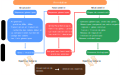
\includegraphics[width=\textwidth]{img/niveaux_annotations.pdf}
        \caption{Présentation des différents niveaux d’annotation.}
        \label{fig:niveaux_annotation}
    \end{shadedfigure}
    
    \subsection{L’évolution des génomes}
    Avant d'approfondir l’annotation génomique, il est nécessaire de comprendre le processus d’évolution des génomes. Car les méthodes d’annotation automatique utilisent cette théorie pour extrapoler des fonctionnalités d’un organisme vers un autre.
    
    Le principe explique que le vivant est soumis à différentes contraintes, environnementale par exemple ( ressources nutritives, température, acidité\ldots ), ainsi avec le temps les générations d’individus les plus adaptés à ces contraintes ont de meilleurs chances de se reproduirent. Par conséquent de transmettre leur patrimoine génétique. D’ailleurs c’est ce patrimoine génétique qui permet de s’adapter aux contraintes. Il est le support de l’expression métabolique et ce métabolisme peut fournir des avantages par rapport aux autres individus. Ainsi tant que métabolisme d’un organisme est adapté à ces contraintes, l’individu peut se reproduire et perpétuer sa lignée génétique.
    
    Toutefois le génome d’un enfant n’est pas forcément la copie exacte des parents. Différents évènements peuvent venir le modifier légèrement. Par conséquent les gènes modifiés vont produire une protéine légèrement différentes. Ces modifications peuvent alors soit procurer un avantage soit un désavantage qui va mener à la fin de la transmission de ce patrimoine. Pour cela, nous observons la plupart du temps seulement les organismes possédant un patrimoine génétique suffisamment adapté à leurs contraintes. En bref, les organismes sous l’effet de pression variées sont sélectionnées.
    
    Suivant cette théorie les gènes se modifient légèrement au cours du temps provoquant de légère modification de leurs séquences. Ainsi des séquences proche de par leur composition sont supposé effectuer produire des protéines avec des fonctions similaires. Le génome peut subir différents évènements qui vont conduire à l’expression de protéines différentes de l’origine. <- mal dit
    
    \begin{shadedfigure}[H]
        \centering
        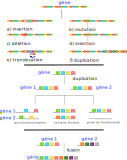
\includegraphics[width=\textwidth]{img/gene_indel.pdf}
        \caption{Présentation de plusieurs évènements génomiques....}
        \label{fig:/evenement_mutation}
    \end{shadedfigure}
    
    En conséquence, les gènes similaires d’organismes différents provenant d’un même gène ancestral sont dit homologues. Par contraste, les gènes d’organismes différents mais n’ayant pas la même origine sont définis comme analogue.
    
    Les évènements de duplications de gènes décrivent la création d’une nouvelle copie de gène dans l’organisme. Étant donné que l'organisme possède une fonctionnalité en double, une des copies peut diverger. En effet, il existe toujours la fonctionnalité originelle sur un gène. La pression de sélection implique qu’une des copies de gène produisent une protéine remplissant la même fonction originelle. On utilise le terme paralogue pour décrire des gènes issue de cet événement de duplication. Un tel évènement peut dupliquer un gène, une région de génome contenant plusieurs gènes  voir dans certains cas un génome.
    
    Les événements de fusion de gène représentent des gènes originellement séparé qui vont former un unique gène. Par opposition les évènements de fission vont  engendrer la coupure d’un gène en deux gènes distincts. Typiquement ce cas est observé avec des gènes codant pour des protéines multi-domaines. Par exemple, une protéine avec deux domaines, codé par un gène se fissure de tels sorte, que chacun des deux nouveaux gènes se spécialise pour produire un des deux domaines de la protéines. Ce phénomène peut engendrer une pression de sélection différentes sur ces deux gènes, selon l’importance du rôle joué par le domaine dans la protéine. Par conséquent un des deux gènes va diverger plus rapidement du gène ancestrale.
    
    Le relâchement de certains facteur de pression de sélection peut conduire à des événements de délétion. L’organisme n’étant plus contraint de posséder une fonctionnalité, les modifications du gène n’impacte pas la capacité de reproduction de l’organisme. Ces modifications peuvent amener à la disparition d’un gène fonctionnel. C’est-à-dire que la séquence du gène à garder des similarités avec le gène ancestrale mais il n’est plus en mesure de fournir la fonctionnalité.
    
    On retrouve également des évènements d’inversion de séquence, de translocations (le gène peut va être déplacé sur un autre chromosome), de transpositions ( un ou plusieurs gènes vont être directement intégré au sein du génome.
    
    L’accumulation de tous ces événements peuvent amener  à une divergence importante du génome par rapport à un génome ancestral. Ceci conduit à l’émergence de nouvelle espèce qui vont évoluer différemment. Ces espèces provenant d’une espèces ancestrales vont avoir des gènes proches. Ces gènes sont dits paralogues.
    
    L’horloge moléculaire des régions qui ne sont pas soumises à la pression de sélection naturelle (ne codant pas pour des gènes) et minimale dans les parties du génome soumises à une forte pression (c'est-à-dire les régions codant pour des fonctions essentielles à la survie de l'organisme).
    
    
    \subsection{Annotation des génomes}
    Changer le contenu de cette section car Annotation fonctionnelle est devenu annotation des génomes.
    Syntaxique, fonctionnelle, relationnelle (dont voies métaboliques) Zoom sur les fonctions impliquées dans les processus bio = voie métaboliques
    
    L’annotation fonctionnelle des gènes, correspond au processus d’attribution de rôle biologique à des gènes. En effet ces gènes vont produire des protéines disposant de une ou plusieurs fonctionnalités pour l’organisme. Ces fonctions sont habituellement classées en trois catégories : moléculaires, cellulaires, phénotypiques.
    
    Les fonctions moléculaires décrivent le rôle biochimique et/ou structural de la protéine. Ainsi les fonctionnalités de catalyse, de liaison et autres sont présentées.
    
    Les fonctions cellulaires établissent les différentes interactions de la protéines au sein de la cellule. Par exemple le rôle d’une enzyme dans une voie métabolique comme la biosynthèse de la lysine . 
    
    Les fonctions phénotypiques détails les caractéristiques observables induite par l’activité d’une protéine. A titre d’exemple, la présence ou l’absence d’une protéine peut jouer un rôle sur la capacité de l’organisme à se développer dans un environnement.
    
    Pour cela l’annotation fonctionnelle basé sur des méthodes expérimentales consiste à isoler chaque produit des gènes afin de tester leurs rôles. Par exemple on peut utiliser un vecteur de clonage contenant un gène d'intérêt. Puis on incorpore le vecteur de dans un organisme. Cet organisme est cultivé afin exprimer le gène d'intérêt. La protéine produit par le gène et ensuite purifier afin d'éliminer tout autre molécule. Et enfin seulement après la réussite des étapes précédentes, on va pouvoir tester les fonctions de la protéine.  Ces méthodes ne sont  pas envisageables à l’état d’un génome. Elles sont utilisées pour valider une prédiction bio-informatique.
    
    Les méthodes d’annotation fonctionnelles  bio-informatiques se base sur la comparaison de séquence. Ainsi les séquences homologues, les protéines de même familles, les séquences possédant un même domaine ou motif partageront des annotations fonctionnelles.
    
    \subsection{Reconstruction des réseaux métaboliques}
    Le métabolisme est un ensemble de réaction biochimique. Une réaction transforme des composés en de nouveaux métabolites. Ces derniers sont modifiés par d'autres transformations. Cette succession d'évènement peut être représenté sous la forme d’un graphe de réactions. Le produit d’une réaction est relié à une autre réaction lorsque cette dernière utilise ce métabolite transformé.
    
    
    \begin{shadedfigure}[H]
        \centering
        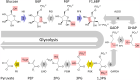
\includegraphics[width=\textwidth]{img/graphe_reactions_glycolyse.pdf}
        \caption{A changer source wikipedia.Représentation de la dégradation du glucose sous forme d’un graphe réactionnel. La  succession des réactions forme un chemin dans le réseau. Cette représentation a pour vocation de restreindre les évènements qui occurrent dans l'organisme aux réactions. Il est important de retenir que ce type de schéma, n'indique pas si ces réactions ont lieu dans le même compartiment cellulaire. Ou encore si les protéines nécessaires aux réactions sont toutes présentes à un moment donné. Cette une vue générale des réactions pouvant avoir lieu dans un organisme.  }
        \label{fig:glycolysis}
    \end{shadedfigure}

    \subsection{Modèles métaboliques}
    \subsection{Les données expérimentales}
    \subsubsection{Élucidation des voies métaboliques}
    Avec la découverte des enzymes à la fin du \siecle{19}, un nouveau champ de connaissance en biologie s’ouvrait. L’enzyme est la clé menant à la compréhension du vivant. Pour cela, la communauté scientifique réalisa un très grand nombre d’expérience permettant produire puis ...
    \subsubsection{Phénotypes de croissances}
    La plupart des molécules biologiques sont constituées d’atome de  carbone (C), d’hydrogène (H), d’oxygène (O), d’azote (N), de phosphore (P) et de soufre (S) (\acrshort{CHONPS}). Par conséquent les organismes doivent avoir au moins une source de nutrition pour chacun de ces éléments. En plus de ces éléments, on considère qu’il est nécessaire pour la vie d’avoir une source de potassium, de calcium, de magnésium, de fer, d’oligo-éléments et d’eau. Ce sont les éléments minimum pour la vie. Tout autre élément permettant à des organismes de se développer est catégorisé comme facteur de croissance. 
    
    Selon les organismes vivants, leurs besoins en éléments et facteurs de croissances varient avec leur capacité métabolique. Ce qui permet de catégoriser les organismes, au regard des manières de constituer de la matière organique via leur anabolisme, ainsi que des moyens de production énergétique via leur catabolisme. (trop lourd) Ces catégories dites types trophiques dépendent de la nature  (i) de la source de carbone (ii) du donneur d’électrons (iii) de la source d'énergie (voir \cref{tab:type trophique}).
    \begin{landscape}
        \begin{table}[H]
            \centering
            \caption{Structuration des différents types trophiques.}
            \label{tab:type trophique}
            \begin{tabular}{|l|l|lr|l|}
            	\hline
                \multirow{2}{*}{\specialcell{Lumière\\\textcolor{orange}{Photo}-}}    					      	&  \multirow{2}{*}{\specialcell{Composé organique\\-\textcolor{nicered}{organo}-}}  & Organique & -\textcolor{psviolet}{hétérotrophe} 	& \textcolor{orange}{Photo}\textcolor{nicered}{organo}\textcolor{psviolet}{hétérotrophe}    \\\cline{3-5}
                                                                                          					  	&                                                               					& Minérale 	& -\textcolor{bleudefrance}{autotrophe}	& \textcolor{orange}{Photo}\textcolor{nicered}{organo}\textcolor{bleudefrance}{autotrophe}  \\\cline{2-5}
                                                                                         					   	&  \multirow{2}{*}{\specialcell{Inorganique\\-\textcolor{brown}{litho}-}}           & Organique & -\textcolor{psviolet}{hétérotrophe} 	& \textcolor{orange}{Photo}\textcolor{brown}{litho}\textcolor{psviolet}{hétérotrophe}     	\\\cline{3-5}
                                                                                            					&                                                               					& Minérale 	& -\textcolor{bleudefrance}{autotrophe}	& \textcolor{orange}{Photo}\textcolor{brown}{litho}\textcolor{bleudefrance}{autotrophe}     \\ \hline
                \multirow{2}{*}{\specialcell{Composé chimique\\organique ou non\\\textcolor{vert}{Chimio}-}}  	&  \multirow{2}{*}{\specialcell{Composé organique\\-\textcolor{nicered}{organo}-}}  & Organique & -\textcolor{psviolet}{hétérotrophe} 	& \textcolor{vert}{Chimio}\textcolor{nicered}{organo}\textcolor{psviolet}{hétérotrophe}   	\\\cline{3-5}
                                                                                            					&                                                               					& Minérale 	& -\textcolor{bleudefrance}{autotrophe}	& \textcolor{vert}{Chimio}\textcolor{nicered}{organo}\textcolor{bleudefrance}{autotrophe}   \\\cline{2-5} 
                                                                                            					&  \multirow{2}{*}{\specialcell{Inorganique\\-\textcolor{brown}{litho}-}}           & Organique & -\textcolor{psviolet}{hétérotrophe} 	& \textcolor{vert}{Chimio}\textcolor{brown}{litho}\textcolor{psviolet}{hétérotrophe}    	\\\cline{3-5}
                                                                                            					&                                                               					& Minérale 	& -\textcolor{bleudefrance}{autotrophe}	& \textcolor{vert}{Chimio}\textcolor{brown}{litho}\textcolor{bleudefrance}{autotrophe}      \\ \hline
            \end{tabular}
        \end{table}
    \end{landscape}
    Certains organismes ont la faculté de se développer dans des milieux dépourvu de facteur de croissance. C’est-à-dire, qu'à partir des éléments minimaux nécessaires à la vie, ils sont capables de produire toutes les molécules  indispensables à leurs développement. Ce sont des organismes dit prototrophe.  Dans le cas contraire on parle d’auxotrophie. 
    
    Le métabolisme fournit les acides aminés indispensables à la production de protéines. Ces protéines sont constituées d’acides aminés. Par conséquent l’organisme doit se procurer ces acides aminés soit par des voies de biosynthèses soit directement par nutrition. C’est pour cela qu’avec les organismes prototrophes on s’attends à retrouver toutes les voies de la biosynthèses des acides aminés. Et par opposition un organisme auxotrophe à un acide aminé ne devrait pas avoir la voie de biosynthèse de ce dernier.
    
    \subsection{MicroScope : une plateforme d’annotation de génomes procaryotes et d’analyse de leur métabolisme}
    
    Chapeau : objectif MicroScope, les différentes publications
    Puis celle de 2017
    Section de la fin : souligner ce qui a été fait en terme de curation pour les bio… mais mieux à faire pour guider les bio dans leur travail de curati=> objectif de ton travail
    
    \includepdf[pages=-]{img/microscope2017.pdf}

    \section{Raisonnement logique dans le processus de curation}
    
    Le processus de curation consiste d’ajouter et/ou enlever des annotations manuellement. Pour cela les bio-curateurs utilisent un ensemble de règles qui leur sont propres. Une des méthodes utilisé par les bio-curateurs passe par la reconstruction des voies métaboliques. Le bio-curateur connaît des caractéristiques phénotypique de son organisme d’intérêt. Il va pour cela commencer par vérifier si les caractéristiques sont corrélés aux prédictions. Par exemple, lorsque l’on reconstruit les voies métaboliques d’un Citrobacter, on s’attend à retrouver au moins une voie complète, permettant la dégradation du citrate. Si ce n’est pas le cas, le bio-curateur informé de cette lacune dans l’annotation, va rechercher un ou plusieurs gènes permettant in-fine d’exprimer cette capacité.
    
    Par ailleurs, lorsque le bio-curateur s’aperçoit qu’il manque une réaction afin de réaliser une voie métabolique. Il va essayer de caractériser le gène en se basant sur le contexte génomique. Les gènes liés aux réactions qui précèdent et succèdent la réaction non annoté à un gène (trop compliqué)
    
    \subsection{Lacunes et incertitudes dans nos connaissances}\label{subsec:lacunes}
    
    Quelque soit le domaine d’expertise, nous avons des éléments imprédictibles par les modèles scientifiques. Notre savoir sur le monde qui nous entoure est encore partiel. Les modèles scientifiques permettent de représenter une partie de ce monde. Mais il existe un nombre de fait, non négligeable, qui échappe à ces  modèles. Ces trous de connaissances peuvent être identifiés lorsque l’on oppose les prédictions aux expectations. Il apparaît que des faits attendues reste non prédit.
    
    D’autre part, les ressources entreposant les faits prédits sont variées. Leurs prédictions proviennent  de différents algorithmes dont leur spécificité \footnote{Proportion de résultat négatifs correctement identifiés.} et sensibilité \footnote{Proportion de résultat positifs correctement identifiés.} diffèrent d’un algorithme à un autre. Ces prédictions aux taux d’erreurs variés viennent enrichir les entrepôts de données. Puis ils seront utilisé à leur tour utilisé pour prédire de nouveau faits. Par conséquent  le taux d’erreur de la première prédiction vient s’ajouter au taux d’erreur de la méthode. Ce processus cyclique, permet de capturer un nombre plus important de fait. Mais il a l’inconvénient de sur-prédire.
    
    Ces problématiques sont retrouvées dans le processus de prédictions de fonction protéiques.
    Pour pallier à ce phénomène des initiatives tente de limiter l’extrapolation abusive faites par les prédicteurs. Par exemple \citeauthor{pfeiffer2015manual}
    
    
    \subsubsection{Les trous dans les connaissances et les enzymes orphelines}
    
    blah blah à écrire
    
    \subsubsection{Limites de l’annotation fonctionnelle et rôle de la curation}
    
    blah blah à écrire
    
    Lors de l'analyse des génomes nouvellement séquencé, le biologiste est souvent confronté à la difficile tâche de vérification de la cohérence des gènes annoté vis-à-vis des connaissances biologiques sur l'organisme étudié. Pour cette raison l'automatisation des règles appliquées par le biologiste permettrais de traiter rapidement une quantité importante d'information.
    
    \subsection{Logique et raisonnement}
    
    La logique est une branche à la fois de la philosophie et des mathématiques. Par exemple son utilisation permet d'instrumentaliser les mots afin de faire ressortir la vérité d'une phrase. Dès l'Antiquité elle fut employé comme un outil pour distinguer un raisonnement concluant d'un non-concluant. \textit{Aristote} formalise une logique à deux énoncés (appelées prémisses ou encore propositions) soumis à approbation. Pour illustrer, la phrase qui suit est constitué de deux prémisses séparées par une virgule et de sa conclusion. \textit{Tous les hommes sont mortels, or Socrate est un homme donc Socrate est mortel}. Ainsi la vérification de la véracité de ces prémisses amènent à une conclusion pouvant être vrai ou fausse. Cette méthode de raisonnement s'appelle le syllogisme.
    
    Avec l'arrivée de l'informatique, la logique amena les méthodes nécessaires pour l'automatisation des choix à effectuer par un ordinateur. La combinaison de ces deux domaines, permet d'inscrire une mécanique de raisonnement et de l'automatiser. Les méthodes avenir vont connaître de grande mutation avec le développement de l'intelligence artificielle. Le raisonnement critique sur une masse de donnée toujours plus importante permettrait d'assister l'Homme dans sa quête de savoir.
    
    
    Avant de commencer, il est important d'introduire du vocabulaire issue de la logique. Tout d'abord il est nécessaire de différencier une proposition et un prédicat.  Une proposition peut être vue comme est une assertion pouvant être vrai ou fausse. Par exemple, la phrase "La capitale de la France est Paris." est une proposition (qui est vrai\ldots). En revanche la phrase "La capitale de mon pays est Paris" est un prédicats car elle contient une variable. En effet, tout dépends de qui est désigné par le terme "mon" si c'est un français le prédicat est vrai sinon il fait faux. Au passage ceci met en exemple, la règle du tiers exclu, si ce n'est pas faux c'est vrai et inversement.
    
    Le calcul des propositions consiste de mettre en relation les propositions afin d'aboutir sur une des deux valeurs de vérité ("VRAI" ou "FAUX"). Ceci implique l'utilisation de connecteur pour exprimer la conjonction et la disjonction (\textit{ET} / \textit{OU}), ainsi que l'expression de la négation (\textit{NON}). Pour illustrer, le calcul des proposition permet de déduire que les deux propositions suivantes sont vrais: "La capitale de la France est Paris et Nice est une ville de France".
    
    On utilisera par la suite le symbole "$\land$" pour le \textit{ET} logique, "$\lor$" pour le \textit{OU} logique et "$\lnot$" pour \textit{NON}. L'implication est représenté par le symbole "$\rightarrow$". 
    
    Le calcul des prédicats du premier ordre (également nommé logique du premier ordre) ajoute une couche d'abstraction par l'utilisation des variables. Par exemple on peut déduire l'expression "Le X est un oiseau" selon de ce qui est désigné par "X". Ainsi l'évaluation des variables forme une proposition. D'après l'expression précédente si "X" désigne un renard: "Le renard est un oiseau" est une proposition fausse. La logique du premier ordre est caractérisé par l'utilisation de: variable, de prédicat, de connecteur logique ( \textit{ET}, \textit{OU} \ldots), de quantificateurs (pour tout: "$\forall$", il existe au moins un \ldots tels que: "$\exists$" ). Cette ensemble de caractéristique permet une grande expressivité de problème logique. Par exemple, pour énoncé, "Pour toute personnes françaises, il existe au moins une personne bordelaise" peut s'écrire de la manière suivante:
    
    \begin{equation*}
        \forall x~estUnePersonne(x) \land \exists x~estFrancaise(x) \land \exists x~estBordelaise(x) \stepcounter{equation}
    \end{equation*}
    
    
    La logique met en relation des éléments autour d'une conjonction ou d'une disjonction. Ce tout forme une clause logique composé d'aux moins deux littéraux et d'un connecteur (i.e $p \land q$ ).
    
    Je vais introduire dans les sections qui suivent différents aspects de la logique, qui m'ont inspiré pour mon travail de recherche. Cette introduction aux différentes logiques est une compréhension du domaine en tant que bio-informaticien. Par conséquent certaines parties pourraient apparaître approximative pour un expert du domaine.
    
    \subsubsection{Les différentes logiques}
    
    La logique est employé sur de multiple problématiques et par conséquence de nombreuses méthodes logiques se sont développées. On retrouve la logique booléenne avec les valeurs de vérité "VRAI" et "FAUX", des logiques multi-valuées pour définir des valeurs de vérités supplémentaires pour désigner toutes choses dont ne peut attribuer les valeurs  "VRAI" et "FAUX", les logiques modales permettant de spécifier des qualités au "vrai".
    
    \paragraph{Logique classique}
    
    Une des méthodes logique usuellement utilisé, par toutes personnes développant des programmes informatiques, est la logique de \textit{Boole}. Elle permet de traiter les expressions composer de deux valeurs puis d'effecteur le calcul des propositions. Pour cela elle représente deux prémisses séparé par un opérateur de liaison (la conjonction \textit{ET} ou la disjonction \textit{OU} ). Le calcul de ces propositions aboutissent aux valeurs de vérité "VRAI" ou "FAUX" \footnote{On associe usuellement la valeur 1 pour "VRAI" et 0 pour "FAUX".}. Ainsi la combinaison deux à deux des propositions avec les opérateurs de liaison produisent les tables de vérités (voir \cref{tab:bool_truth_table}). Également l'algèbre de \textit{Boole} définit l'opérateur de négation \textit{NON}. Il permet d'inverser les valeurs de vérité. Une proposition "NON VRAI" est "FAUX" et inversement. Les opérateurs logique \textit{ET} et \textit{OU} sont dit binaire car ils impliquent deux opérandes, par opposition \textit{NON} est unaire.
    
    
    \begin{table}[H]
        \centering
        \caption{Table de vérité utilisant l'algèbre de \textit{Boole}. La lettre "T" désigne la valeur de vérité "VRAI" et "F" pour "FAUX". }
        \label{tab:bool_truth_table}
        \begin{subtable}{0.5\linewidth}
            \centering
            \caption{A et B sont deux propositions dont on attribue tour-à-tour différentes valeurs de vérité.}
            \begin{tabular}{|>{\columncolor{LightCyan}}l|>{\columncolor{LightCyan}}l|l|l|}
                \toprule
                \rowcolor{LightCyan}
                A   &   B   & $A \land B$               & $A \lor B$                \\
                \midrule
                T   &   T   & $T \land T \rightarrow T$ & $T \lor T \rightarrow T$  \\ \hline
                T   &   F   & $T \land F \rightarrow F$ & $T \lor F \rightarrow T$  \\ \hline
                F   &   F   & $F \land F \rightarrow F$ & $F \lor F \rightarrow F$  \\
                \bottomrule
            \end{tabular}
        \end{subtable}
        \begin{subtable}{0.35\linewidth}
            \centering
            \caption{Calcul de la proposition A avec l'opérateur "NON".}
            \begin{tabular}{|>{\columncolor{LightCyan}}l|l|}
                \toprule
                \rowcolor{LightCyan}
                A   &  $\lnot A$ \\
                \midrule
                T   & $\lnot T \rightarrow F$ \\ \hline
                F   & $\lnot F \rightarrow T$ \\
                \bottomrule
            \end{tabular}
        \end{subtable}
    \end{table}

    La logique classique ne se limite pas à l'algèbre de \textit{Boole}. Elle recherche à classé le monde en vrai/faux. Par exemple Georg Cantor un éminent logicien du \siecle{19} initia la théorie des ensembles \cite{cantor1879satz}. Elle permet d'utiliser les opérateurs logique \textit{ET},\textit{OU},\textit{NON} sur des ensembles. Et ainsi de déterminer les éléments appartenant ("$\in$") ou non ("$\notin$") à un ensemble. Pour illustrer, deux ensembles A et B, les éléments correspondant à l'ensemble A "ET" à l'ensemble B sont les éléments présent à l'intersection de ces deux ensembles. Lorsque l'on recherche les éléments présents dans A ou B correspond ceci corresponds à rechercher dans l'ensemble former par l'union de ces deux ensembles. Et enfin lorsque l'on recherche à exclure un ensemble on utilise l'opérateur \textit{NON} ce qui se traduit par le complément de cet ensemble (voir \cref{fig:ensemble}).
    
    
    \begin{shadedfigure}[H]
        \centering
        \caption{Différentes opérations ensemblistes sélectionnées par la couleur cyan.}
        \label{fig:ensemble}
        
        \begin{subfigure}{0.45\linewidth}
            \centering
            \caption{Ensemble A}
            \begin{tikzpicture}[scale=0.45,background rectangle/.style={fill=white}, show background rectangle]
                \tkzDefPoint(0,0){A}  
                \tkzDefPoint(4,0){B}
                \tkzDrawCircle[fill=Cyan,color=Cyan](A,B)  
                \tkzLabelPoints[below](A)
            \end{tikzpicture}  
        \end{subfigure}
        \begin{subfigure}{0.45\linewidth} 
            \centering
            \caption{Complement de l'ensemble A: $\lnot A$}
            \begin{tikzpicture}[scale=0.45,background rectangle/.style={fill=Cyan}, show background rectangle]
            \tkzDefPoint(0,0){A}  
            \tkzDefPoint(2,0){B}
            \tkzDrawCircle[fill=white](A,B)  
            \tkzLabelPoints[below](A)
            \tkzLabelCircle[R,text width=2cm,text centered](A,3 cm)(-70){NON A}
            \end{tikzpicture}
        \end{subfigure}
        \vskip 8pt
        \begin{subfigure}{0.45\linewidth}
            \centering
            \caption{Intersection de l'ensemble A et B: $A \cap B$}           
            \begin{tikzpicture}[scale=0.45,background rectangle/.style={fill=white}, show background rectangle]
            \tkzDefPoint(0,0){A}  
            \tkzDefPoint(4,0){B}
            \begin{scope}
            \tkzClipCircle(A,B) \tkzClipCircle(B,A)
            \tkzFillCircle[color=Cyan](A,B)  
            \end{scope}
            \tkzDrawCircle(A,B)  
            \tkzDrawCircle(B,A)
            \tkzLabelPoints[below](A,B)
            \end{tikzpicture}  
        \end{subfigure}
        \begin{subfigure}{0.45\linewidth}
            \centering
            \caption{Union de l'ensemble A et B: $A \cup B$}           
            \begin{tikzpicture}[scale=0.45,background rectangle/.style={fill=white}, show background rectangle]
            \tkzDefPoint(0,0){A}  
            \tkzDefPoint(4,0){B}
            \tkzDrawCircle[fill=Cyan,color=Cyan](A,B)  
            \tkzDrawCircle[fill=Cyan,color=Cyan](B,A)
            \tkzLabelPoints[left](A)
            \tkzLabelPoints[right](B)
            \end{tikzpicture} 
        \end{subfigure}
        
    \end{shadedfigure}

    La théorie des ensembles tel qu'énoncé par \textit{Georg Cantor}, laissait apparaître des paradoxes comme le paradoxe de Russell ("\textit{l'ensemble des ensembles n'appartenant pas à eux-mêmes appartient-il à lui-même ?}"), le paradoxe du plus grand cardinal \footnote{Un ordinal caractérise une liste ordonnée et un cardinal caractérise une quantité d'objet.} et d'autres \ldots~. Pour cela la théorie des ensembles a été axiomatisé \footnote{Procédé pour déduire de façon logique et rigoureuse un théorème.} en logique du premier ordre par \textit{Ernst Zermelo}, \textit{ Abraham Fraenkel} et \textit{Thoralf Skolem} \cite{hayden1968zermelo,kanamori2008higher}. La théories des ensembles de Zermelo-Fraenkel (abrégé ZF) apporte la notion de classe pour représenter des collections d'objet partageant une ou plusieurs propriétés , mais cette collection d'objet ne forme pas un ensemble. Cette notion de classe permet de lever les ambiguïtés et donc les paradoxes originelles liée à la théories des ensembles de \textit{Georg Cantor}. Toutefois il existe des théories voisines de la ZF comme la théorie des classes \cite{bernays1937system,van1967frege} de \textit{von Neumann-Bernays-Gödel} (NBG).

    \citation{"Grandeurs" : Voilà un mot dont tout le monde croit avoir une idée bien nette et qu'il est assez difficile de bien définir. Ne serait-ce pas parce que l'idée que ce mot renferme est plus simple que les idées par lesquelles on peut entreprendre de l'expliquer ? }{Jean Rond d'Alembert}
        
    \paragraph{Logique multivaluée}\label{par:logic_multivalué}
    
    Les logiques multivaluées recherche à étendre le vocabulaire pour déterminé la véracité d'une expression. Parfois il est nécessaire d'assigner un état autre que vrai ou faux. Lorsque l'on souhaite exprimer l'incertitude, on ne peut pas asserter par un état vrai ou faux. Car cela reviendrait à mettre un affirmation ou une infirmation sur l'expression. Par conséquent de tels logiques ne peuvent plus employer la règle du tiers exclu.
    
    Pour cela des logiques à trois valeurs de vérité sont employées, comme la logique de \textit{Kleene} (K$_{3}$) ou encore celle de \textit{Priest} P$_{3}$. La logique K$_{3}$ utilise la troisième valeur de vérité pour signifier un état indéterminé (noté I).  Cette nouvelle valeur représente ce qui est ni vrai ni faux.  Tandis que dans la logique P$_{3}$ la troisième valeur représente l'état vrai et faux permettant l'expression d'une contradiction. Malgré cette différence ces deux logique se représente à travers les mêmes table de vérité (voir table de vérité \ref{tab:three_truth_table}).
    
    
    \begin{table}[H]
        \centering
        \caption{Table de vérité pour la logique de Kleene (strong)K$_{3}^{s}$  }
        \label{tab:three_truth_table}
        \begin{subtable}{0.2\linewidth}
            \centering
            \begin{tabular}{|>{\columncolor{LightCyan}}l|l|}
                \toprule
                \rowcolor{LightCyan}
                $\lnot$ &    \\
                \midrule
                T       &   F\\ \hline
                I       &   I\\ \hline
                F       &   T\\
                \bottomrule
            \end{tabular}
        \end{subtable}
        \begin{subtable}{0.35\linewidth}
            \centering
            \begin{tabular}{|>{\columncolor{LightCyan}}l|l|l|l|}
                \toprule
                \rowcolor{LightCyan}
                $\land$ & T & I & F \\
                \midrule
                T       & T & I & F \\ \hline
                I       & I & I & F \\ \hline
                F       & F & F & F \\
                \bottomrule
            \end{tabular}
        \end{subtable}
        \begin{subtable}{0.35\linewidth}
            \centering
            \begin{tabular}{|>{\columncolor{LightCyan}}l|l|l|l|}
                \toprule
                \rowcolor{LightCyan}
                $\lor$ & T & I & F \\
                \midrule
                T       & T & T & T \\ \hline
                I       & T & I & I \\ \hline
                F       & T & I & F \\
                \bottomrule
            \end{tabular}
        \end{subtable}
    \end{table}

    \textit{Belnap} combine la logique K$_{3}$ et P$_{3}$ afin de pouvoir discriminer l'inconnu et la contradiction.  Pour cela il définit la valeur ni vrai ni faux de \textit{Kleen} par une valeur signifiant "aucun" état ("None"). Et pour la valeur vrai et faux exprimé par \textit{Priest}, il utilise l'état "les deux" ("Both"). À partir de ces quatre valeurs de vérité (Vrai, Faux, Aucun, Les deux), \textit{Belnap} décrit une logique pour gérer des informations dont on ne peut pas statuer simplement en vrai/faux. Cette logique est également noté B$_{4}$ \cite{belnap77}. La table de vérité associé est présenté dans le \cref{tab:belnap_truth_table}) . 
   
    
    \begin{table}[H]
        \centering
        \caption{Table de vérité pour la logique B$_{4}$. La lettre N représente ce qui est non déterminé et la lettre B ce qui est vrai-et-faux.  }
        \label{tab:belnap_truth_table}
        \begin{subtable}{0.2\linewidth}
            \centering
            \begin{tabular}{|>{\columncolor{LightCyan}}l|l|}
                \toprule
                \rowcolor{LightCyan}
                $\lnot$ &    \\
                \midrule
                T       &   F\\ \hline
                B       &   B\\ \hline
                N       &   N\\
                F       &   T\\
                \bottomrule
            \end{tabular}
        \end{subtable}
        \begin{subtable}{0.35\linewidth}
            \centering
            \begin{tabular}{|>{\columncolor{LightCyan}}l|l|l|l|l|}
                \toprule
                \rowcolor{LightCyan}
                $\land$ & T & B & N & F \\
                \midrule
                T       & T & B & N & F \\ \hline
                B       & B & B & F & F \\ \hline
                N       & N & F & N & F \\ \hline
                F       & F & F & F & F\\
                \bottomrule
            \end{tabular}
        \end{subtable}
        \begin{subtable}{0.35\linewidth}
            \centering
            \begin{tabular}{|>{\columncolor{LightCyan}}l|l|l|l|l|}
                \toprule
                \rowcolor{LightCyan}
                $\lor$ & T & B & N & F \\
                \midrule
                T       & T & T & T & T \\ \hline
                B       & T & B & T & B \\ \hline
                N       & T & T & N & N \\ \hline
                F       & T & B & N & F\\
                \bottomrule
            \end{tabular}
        \end{subtable}
    \end{table}

    Ces travaux sur une logique à plusieurs valeurs s'intègre plus généralement dans ce que l'on appelle la logique paracohérente ("Paraconsistent Logic"). L'intérêt de ces approches et de pouvoir raisonner sur des informations incohérente et incomplètes sans tomber dans de l'absurde. Dans une logique non paracohérente, lorsqu'une incohérence est rencontré, \textit{de facto} tout ce qui est obtenu à partir de cette information est incohérente à son tour. Ainsi soit l'information n'est pas traité soit elle celui est assimilé à de la fausseté. Par conséquent la notion de faux n'indique plus seulement la certitude d'une fausseté mais également l'inconnu et la contradiction.
    
    Finalement la paracohérente logique est une méthode de raisonnement permettant de mettre en lumière les absurdités, les certitudes et ce qui reste d'inconnu. Surtout dans un monde ou l'information est multiple. Nous ne pouvons pas garantir ça cohérence vis à vis des autres informations. Par opposition en logique classique afin de garantir la cohérence des résultats il est nécessaire de certifier qu'il n'existe pas d'ambiguïté dans les information avant de comment un raisonnement. Ce qui n'est pas toujours faisable \ldots
    
    On retrouve d'autres logiques cherchant à décrire les combinaisons de ces quatre valeurs de vérité. Ainsi l'agrégation de ces valeurs de vérité forme de nouvelle valeur. Comme dans la logique à seize valeurs décrit par \citeauthor{shramko2005some} \cite{shramko2005some,shramko2011truth,shramko2006hyper}. La combinaison des valeurs T (Vrai) et B (les deux) forme la valeur TB (voir \cref{fig:sixteen_truth_values}). Ces nouvelles valeurs de vérité sont pour \citeauthor{shramko2005some} une généralisation des valeurs décrites par \textit{Nuel Belnap}. Ces valeurs généralisées représente des ensembles de valeur de vérité. La valeur TF par exemple est un ensemble constitué de l'ensemble T et de l'ensemble F : $\{\{t\},\{f\}\}$. Alors que la valeur B est un ensemble de valeur vrai et faux: $\{t,f\}$. Cette structure mathématique permet d'ordonner les valeurs de vérité via des opérations ensemblistes. Pour cela \textit{Shramko et al} définissent une méthode pour ordonner les valeurs de vérité entre elles selon l'échelle de l'information (\ref{eq:sixteen_definition_info}), la véracité (\ref{eq:sixteen_definition_truth}) ou encore celui de la fausseté (\ref{eq:sixteen_definition_falsehood}) . Les méthodes pour la comparaison sur l'ordre de la véracité et de la fausseté pose le postulat que T et F sont respectivement le maximum pour chacun des deux ordres. Pour cela la méthode consiste à créer deux ensembles (x$^{t}$ et x$^{-t}$) pour chaque valeur de vérité à comparé. Tels que x$^{t}$ est un sous-ensemble de x contenant $\{t\}$ et x$^{-t}$ un sous ensemble de x à l'exclusion de $\{t\}$. La même méthode est appliqué pour la fausseté en utilisant le sous ensemble $\{f\}$.  C'est une méthode comparative deux à deux. Par conséquent elle ne permet pas de positionner unitairement, une valeur de vérité selon un degrés de véracité ( de même pour la fausseté et l'information) .
    
    \textbf{Définition:} Pour tout x,y parmi les valeurs de vérité en Sixteen$_{3}$:\nolisttopbreak \vspace{-0.5cm}
    \begin{align}
        \begin{split}
        x \leq& _{i} \, y \; \iff \: x \subseteq y\label{eq:sixteen_definition_info};
        \end{split}\\ \begin{split}\label{eq:sixteen_definition_truth}
        x \leq& _{t} \, y \; \iff \: x^{t} \subseteq y^{t} and \, y^{-t} \subseteq x^{-t},\\
              &where \; x^{t} := \{z \in x | t \in z \} \, and \, x^{-t} := \{z \in x | t \notin z \};
        \end{split}\\ \begin{split}\label{eq:sixteen_definition_falsehood}
        x \leq& _{f} \, y \; \iff \: x^{f} \subseteq y^{f} and \, y^{-f} \subseteq x^{-f},\\
              &where \; x^{f} := \{z \in x | f \in z \} \, and \, x^{-f} := \{z \in x | f \notin z \};
        \end{split}
    \end{align}
    
    Description des symboles:\nolisttopbreak
    \begin{itemize}
        \item t et f sont respectivement le vrai et le faux de la logique classique
        \item $\iff$ désigne: si et seulement si
        \item $x \subseteq y$ pour indiquer que  l'élément x est ou un sous-ensemble voire un ensemble identique à y
        \item $x \in y$ pour informer que l'élément x appartient à l'ensemble y et  $\notin$ pour n'appartient pas
        \item $E : \{ x \in \mathbb{N} | x < 10 \}$ pour définir un ensemble ($\{\}$) E contenant des nombres entiers naturel ($\mathbb{N}$) nommé x tels que($|$) tout x est strictement plus petit que 10
        \item z est un sous ensemble de la valeur de vérité
    \end{itemize}

    \textbf{Exemple:} Pour x: NTF $\{\{\emptyset\},\{t\},\{f\}\}$ et y: B $\{\{t,f\}\}$:\nolisttopbreak \vspace{-0.5cm}
    \begin{equation*}
    \begin{rcases}
    x^{t}  := \{ \{t\} \}               &y^{t}  := \{ \{t,f\} \}\\
    x^{-t} := \{\{\emptyset\},\{f\} \}  &y^{-t} := \{ \{\emptyset\} \} \\
    \end{rcases}
     \{ \{t\} \} \subseteq \{ \{t,f\} \} \land \{ \{\emptyset\} \} \subseteq \{\{\emptyset\},\{f\} \}
    \end{equation*}


    \begin{shadedfigure}[H]
        \centering
        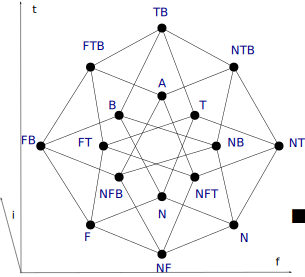
\includegraphics[width=0.6\textwidth]{img/Generalized_Truth_Values_and_Multilattices.pdf}
        \caption{ Treillis issue de la combinaison des valeurs de vérité (T,F,B,N). L'agrégation de toutes les valeurs de vérité est représenté par la lettre A ("all"). Cette figure représente les valeurs de vérité selon trois axes, (i) la vérité "t", (ii) la fausseté "f$^{-1}: t -f $", (iii), l'information noté "i". Ce treillis est appelé par \textit{Shramko et al.} "Trilattice Sixteen$_{3}$".  }
        \label{fig:sixteen_truth_values}
    \end{shadedfigure}

    \paragraph{Logique modale}
    La Logique modale est une extension de la logique propositionnelle. Elle permet de raisonner sur l'incertain et les situations évolutives. Pour cela la sémantique est plus expressive. Elle permet de moduler la notion de véracité avec des notions comme obligatoire $\square$ et concevable $\diamond$. Ainsi on peut émettre des propositions plus nuancés pour recherché si elle sont vrais dans certains cas de figure. La véracité d'une proposition va être recherché dans des "mondes possibles". Typiquement lorsqu'on lance une pièce de monnaie. (i) La pièce est obligatoirement du côté PILE ou FACE. (ii) Obtenir le côté PILE est possible tout comme FACE. (iii) Et elle ne peut être PILE et FACE en même temps. On comprend que les côté PILE et FACE sont deux mondes accessibles. Ils ne peuvent pas être tous les deux vrais dans un même monde (i.e pour une même pièce à un même instant).
    
    Ceci est généraliser de la façon suivante:\nolisttopbreak
    \begin{enumerate}[label=\roman*)]
        \item $\square A$ est vraie dans un monde possible ω si A est vraie dans tous les mondes possibles accessibles à partir de ω.
        \item $\diamond A$ est vraie dans un monde possible ω si A est vraie dans au moins un monde possible accessible à partir de ω.
        \item $\square A \land \square B$ est obligatoirement faux dans un monde ω si $\square A \to \lnot \square B \lor \square B \to \lnot\square A$
    \end{enumerate}

    La logique modale permet d'exprimer quatre notions ( plus en les combinant ):
    \begin{enumerate}[label={}]
        \item $\square p$: p est nécessaire / obligatoire
        \item $\lnot\square p$: p est contingent / incertain
        \item $\diamond p$: p est possible / concevable
        \item $\lnot \diamond p$: p est impossible
    \end{enumerate}

    Il existe une multitude de logique modale comme les logiques temporels, épistémiques, déontiques ou encore les logiques alétiques. Chacune d'elles apporte une nuance aux différentes modalités ($\square \diamond$).
    
    \begin{tabular}{ll}
        temporels:      & il va faire un beau temps \\
        épistémiques:   & l'agent sait qu'il fait un beau temps,  l'agent croit qu'il fait un beau temps \\
        déontiques:     & il doit faire un beau temps \\
        alétiques:      & il est possible qu'il fasse un beau temps \\
    \end{tabular}

    Bien que je n'ai pas travaillé sur la logique modale en tant que tel. J'ai le sentiment que le travail de recherche effectué à travers GROOLS peut avoir des liens avec la logique modale. Notamment au travers des notions: "requis", "interdit", "incertain" et "peut être" utilisé pour la formulation des conclusions. Mais également avec les notions de prédiction et d'expectation. Elles ont un sens proche de ce qui est exprimé en logique épistémiques ("on croît" / "on sait"). Mais également sur les conclusions "La connaissance doit être manquante" semble une formulation proche de la logique déontiques.
    
    
    
    \subsubsection{Logique de description}
    
    C'est un domaine de la logique utilisé pour établir des faits en utilisant une représentation structurée de la connaissance. La logique de description est une composante de l'intelligence artificielle. Car cette dernière nécessite de représenter les connaissances afin de pouvoir calculer/déduire de nouveau savoir. Dans les grandes lignes, ce domaine s'attache à caractériser les catégories d'objets puis de les mettre en relation. La représentation des connaissance et le raisonnement appliqué sur ces connaissances permettent la construction d'application intelligente. En référence à la capacité d'un système de trouver des conséquences implicites à partir de connaissance explicite.
    
    Une telle structuration des connaissances forme un réseau dont les individus sont des concepts (les nœuds) exposant différents type de lien. Le mot terminologie est employé dans ce domaine pour décrire les intentions données lors de la construction d'une structure hiérarchique. Et la sémantique utilise la terminologie pour étudier de qui est signifié.
    
    \paragraph{Représentation des connaissances}
    La structuration hiérarchique des connaissances permet une représentation compacte et compréhensible de l'information. Mais surtout elle permet d'appliquer un raisonnement logique sur ces connaissances.
    
    Par exemple une structuration hiérarchique de concept relié les uns aux autres par des relations symbolisant le "ET" et le "OU" sont efficacement disposé lorsque l'arbre est une disjonction de clause.
    En effet dans de tels cas on peut rechercher indépendamment la véracité de l'un ou de l'autre littéral. Il suffit d'établir qu'un des deux littéral soit vrai pour déduire que la clause est vrai à son tour. Une telle structuration est une forme normale disjonctive.
    
    Évidement la logique de description n'est pas limité aux relations ET/OU. Des sémantiques comme celle proposé par \acrfull{GO}, dispose de relation pour exprimer la composition et l'identité. Pour cela  \acrfull{GO} propose un vocabulaire contrôlé (l'ontologie). On ne peut pas parlé de la représentation des connaissances sans cité le web sémantique (standardisé par le W3C \footnote{W3C, est un organisme de standardisation à but non lucratif, fondé en octobre 1994 chargé de promouvoir la compatibilité des technologies du World Wide Web.}). Le web sémantique incarne un effort important de la communauté à fournir les outils et les méthodes pour analyser l'information dans sons sens le plus générale. Une fois l'information structuré, des méthodes de raisonnement sur ces données peuvent être appliquées.
    
    \paragraph{Chaînage avant et arrière} %backward/forward
    Un raisonnement peut être décrit par une suite de règle. Une tel règle comporte deux partie. La première partie sélectionne les informations correspondant à une contrainte. Comme par exemple: "x est une transaminase", tous faits respectant la contrainte seront sélectionnés. Puis la deuxième partie correspond au conséquence logique. Pour faire suite à l'exemple précédent: "alors x est une protéine" . Ces deux parties forme une règle d'inférence. Les conséquences logiques d'une règle peuvent activer de nouvelles règles. Par la méthode du chaînage avant, les faits (des prémisses) sont utilisés pour remonter aux conclusions. Ce processus de déduction se poursuit tant qu'il existe des faits respectant les contraintes des règles.
    
    Prenons les trois règles suivantes:\nolisttopbreak    
    \begin{enumerate}
        \item Si x est une transaminase alors x est une protéine
        \item Si x est un ARN alors x est composé d'acides ribonucléiques
        \item Si x est une protéine alors x est composé d'acides aminés
    \end{enumerate}

    Lorsque le moteur d'inférence traite le fait "aspartate aminotransférase". La règle \ding{172} est activé et  conclut que le fait est une protéine. Cette conséquence va permettre d'activer à son tour la règle \ding{174} et conclure sur ça composition. Aucun fait restant peut activer une règle, fin du raisonnement.
    
    Il est possible également de partir des conclusions pour revenir aux prémisses, par la méthode du chaînage arrière. Ces méthodes de chaînage sont mis en œuvre à travers des moteurs d'inférence.
    
    \paragraph{Système expert} la mise bout à bout des connaissances, des règles d'inférence et des faits observés permet de reproduire des systèmes cognitif d'un expert d'un domaine (bio-curateur par exemple). Cet ensemble forme un système expert, ce procédé est utilisé notamment pour la mise en œuvre de l'intelligence artificielle. Pour cela, un tel système dispose d'une base de fait, une base de règle et un moteur d'inférence. Les déductions effectuer à partir des faits observé permettent dans certains d'acquérir de nouvelles connaissances. Ce qui se traduit par la formulation de nouvelle règle. Cet apprentissage automatique permet de dépasser le cadre théorique imposé par les règle de départ. Afin de mimer un comportement d'un expert faisant preuve d'adaptabilité face aux problèmes.
    
    \section{Méthodes existantes}
    
    Dans le domaine de la biologie et plus précisément sur l'annotation des gènes, il existe plusieurs ressource utilisant des systèmes à base de règle. Ce qui nous amène à présenter UniRule, Genome properties et IMG terms. Comme expliqué par \citeauthor{dale2010machine}\cite{dale2010machine} il ne faut pas perdre le point de vue suivant, l'annotation des gènes est essentiel pour étudier le réactome d'un organisme.
    
    \subsection{UniRule}
    Dans l'objectif de mimer l'expertise humaine sur l'annotation de plusieurs milliard de séquence, UniProt à mis en place un outil à base de règle appelé UniRule \cite{unirule2015,bridge2010unirule}. C'est une base de règle unifiant les règles provenant d'\gsl{HAMAP}, \gsl{PIR} et RuleBase . UniRule est utilisé conjointement avec \acrfull{SAAS} \cite{kretschmann2001automatic,uniprot2015} pour l'annotation des protéines (voir Figure~\cref{fig:unirule}).
    
    \begin{shadedfigure}[H]
        \centering
        \includegraphics[width=\textwidth]{img/unirule.png}
        \caption{ Chaînage d'application pour l'annotation automatique pour la base de donnée UniProtKB. Figure extraite de \citetitle{bridge2010unirule}. }
        \label{fig:unirule}
    \end{shadedfigure}

    Les règles \acrshort{PIR} proviennent de deux bases de règle.  Celle regroupant les règles d'annotation des sites protéiques (\acrfull{PIRSR} \cite{vasudevan2011structure}) et celle du nommage (\acrfull{PIRSN}). Les règles \acrfull{PIRSR} sont validé humainement. Ces règles d'annotation ont une précision atomique. C'est à dire que la composition de la séquence protéique est utilisable pour déclencher une règle.
    
    En ce qui concerne \acrfull{HAMAP}, c'est un système automatique de classification et d'annotation des séquences protéiques. Il est maintenu par le groupe Swiss-Prot . Pour cela, \acrfull{HAMAP} se base sur des profiles de séquences protéiques validé par l'Homme et également des règles d'annotation fonctionnelle créer par des experts du domaine. La syntaxe des règles  \acrfull{HAMAP} permet une grande expressivité et utilise le vocabulaire contrôlé d'UniProt et les termes \acrfull{GO} (présenté dans \url{http://hamap.expasy.org/unirule/unirule.html}). Tout comme les règles provenant de \acrfull{PIR}, \acrfull{HAMAP} peut effectuer des choix d'annotations selon la composition de la séquence protéique. Cela permet de déclarer des résidus clef, nécessaire pour effectuer une annotation fonctionnelle. Et ainsi, d'être un des moyens de stopper la propagation des erreurs d'annotations persistante dans les ressources publiques \cite{schnoes2009annotation,devos2001intrinsic,bell2013can,gilks2002modeling}. Les annotations amené par \acrfull{HAMAP} concerne de nombreux champs comme: la protéine, le nom du gène, les fonctions, les activités catalytiques, la localisation intracellulaire, les interactions protéines-protéines. Le système classifie automatiquement les séquences dans une des familles validé par les bio-curateurs en utilisant l'homologie de séquence.
    
    \subsection{Genome properties}
    
    Cette ressource part du constat qu'il ai plus aisé d'annoter les protéines lorsqu'elles sont mises dans un contexte métabolique. Les informations de présence/absence de voie métabolique ou encore la structuration de cette dernière fournisse de précieuse information pour l'annotation des protéines. Ainsi \texttt{Genome Properties} \cite{selengut2007tigrfams,haft2005genome,haft2013tigrfams} à regroupé les systèmes clefs d'un organisme prokaryotique dans une structuration hiérarchique (voir Figure~\cref{[fig:gp_lysine]}). À travers un vocabulaire contrôlé les propriétés reflètent le: contenu en gène, phénotype, phylogénie et analyses computationnel (comme les chaîne issue de \acrfull{HMM}). Par déduction les prédictions bioinformatique vont prédire la présence des gènes. Ces derniers permettent de déduire un phénotype. par conséquent elle n'est pas restreinte à la génération de voie métabolique. L'approche permet \textit{in fine} une comparaison entre organisme des fonctionnalités métaboliques et de mettre en lien les protéines non caractérisés.
    
    \begin{shadedfigure}[H]
        \centering
        \includegraphics[width=\textwidth]{img/lysine_biosynthesis.pdf}
        \caption{ Représentation graphique de l'organisation des données au sein de genome properties. Au centre la voie métabolique de la biosytnthèse de la lysine via l'utilisation du diaminopimelate. }
        \label{fig:gp_lysine}
    \end{shadedfigure}

    Les données de genome properties sont extraites de la ressource \acrfull{CMR} \cite{peterson2001comprehensive,davidsen2009comprehensive}. Ces données d'entrées sont issue soit de la recherche de \texttt{TIGRFAM} \cite{haft2003tigrfams}\label{key} soit de la recherche de séquence discriminante représenter par des \texttt{Pfam} \acrfull{HMM} \cite{bateman2000pfam,bateman2002pfam,bateman2004pfam,finn2008pfam,finn2009pfam,punta2011pfam,finn2013pfam,finn2016pfam}. Ces données sont considérées comme des preuves dans la structure de \texttt{Genome Properties}. Elles sont relié à des composants. Les composants sont les briques du systèmes, elles sont utilisés pour regroupé des notions entre elles pour représenté une propriété (notion plus généraliste). Par exemple un ensemble de gènes représentant un des chemins métabolique pour produire un composé d'intérêt pour l'organisme. Ainsi la hiérarchie est une suite de preuve - composant - propriété qui se répète (voir Figure~\cref{fig:gp_modele}).
    
    \begin{shadedfigure}
        \tikzset{
            treenode/.style = { shape=rectangle     , rounded corners,
                                draw, align=center  ,
                                top color=white     , bottom color=blue!20},
            root/.style     = {treenode, font=\Large, bottom color=red!30},
            other/.style    = {treenode, font=\ttfamily\normalsize},
        }
        \begin{tikzpicture}
        [
            grow                    = down,
            sibling distance        = 16em,
            level distance          = 5em,
            edge from parent/.style = {draw,color=black, -latex, <-},
            every node/.style       = {font=\footnotesize,color=black},
            execute at end picture=%
            {
                \begin{pgfonlayer}{background}
                \path[fill=white]
                (current bounding box.south west) rectangle
                (current bounding box.north east);
                \end{pgfonlayer}
            }
        ]
        \node[root]{Property}
            child { node [other] {Component}
                child { node [other] {Evidence}
                    child{ node [root] {Property}
                        child{ node [other] {Component}
                            child { node [other] {Evidence}
                                edge from parent node [above right]  {sufficient for} }
                            node[above right=0.2em and 3em,color=blue,font=\tiny]{is dispensable*}
                            edge from parent node [above,sloped] {part of}}
                        child{ node [other] {Component}
                            child { node [other] {Evidence}
                                edge from parent node [above right]  {sufficient for} }
                            edge from parent node [above,sloped] {part of}}
                        edge from parent node [above right]  {is a} }
                    edge from parent node [above right]  {sufficient for} }
                edge from parent node [above,sloped] {part of} }
            child { node [other] {Component}
                child { node [other] {Evidence}
                    edge from parent node [above right]  {sufficient for} }
            edge from parent node [above,sloped] {part of} };
            
            
        \end{tikzpicture}
        \caption{Modèle de la structure hiérarchique utilisé pour représenter les concepts au sein de \texttt{Genome Properties}. En plus de la structure des méta-informations comme le fait d'indiquer un composant facultatif ("dispensable").  }
        \label{fig:gp_modele}
    \end{shadedfigure}
    
    \subsection{IMG terms}
    
    \texttt{IMG terms} \cite{chen2013improving} est certainement la méthodologie la plus proche de celle utilisé par \texttt{GROOLS}. La méthodologie employé recherche à être robuste aux données biologiques  erronées. Comme nous l'avons vu dans la section \nameref{subsec:lacunes} les données biologiques dans les ressources publiques sont partielles et contradictoires. Pour cela le raisonnement emploie une logique tri-valué. Bien que non déclaré comme tel dans l'article "\citetitle{chen2013improving}", ce sont les mêmes table de vérité que celles décrites par \textit{Kleen} et \textit{Priest} (présenté dans la partie \nameref{par:logic_multivalué}). Le raisonnement appliqué attribue aux voies métaboliques un des trois états vrai, faux, inconnu.
    
    Tout d'abord les \texttt{IMG terms} forment un vocabulaire contrôlé. Ils sont notamment utilisés pour décrire des \texttt{IMG reaction}  et des \texttt{IMG pathway}. Les \texttt{IMG reaction} représente des réactions généralisés, c'est-à-dire qu'une \texttt{IMG reaction} peut correspondre à plusieurs réactions. Ce qui permet de fusionner les réactions alternatives à une \texttt{IMG reaction}. Chaque réaction est relié à une ou plusieurs \texttt{IMG reaction}. La présence d'une \texttt{IMG reaction} est considéré comme présente lorsqu'au moins un des réactions alternatives possèdent tous les \texttt{IMG terms} impliqués dans ça réactions. Ainsi sont assignés aux \texttt{IMG reaction} un des trois états: certifié ("asserted") de celles inconnu("unknown") et non certifié ("not asserted"). À partir de l'état des \texttt{IMG reaction} composant un  \texttt{IMG pathway}, l'état de la voie métabolique est déduit par simple calcul des propositions. En effet les "règles" d'inférence sont représentées ici sous la forme de conjonction et disjonction de réaction:
    
    \begin{equation}
        IMG_{reaction1} \, AND \, (IMG_{reaction2} \, OR \, IMG_{reaction3} ) \to IMG_{pathway 1}
    \end{equation}
    
    \textbf{Ce qui suit doit peut être déplacé en discussion.}
    
    Toutefois la méthode utilisé reste assez flou, la distinction entre prédiction et expectation s'entre mêle. La combinaison de deux états (provenant de : certifié, inconnu, non certifié) implique neuf combinaisons possibles. Mais ces combinaisons sont représentables uniquement par les valeurs vrai,faux,inconnu. Donc un même résultat peut correspondre à plusieurs combinaisons. Ce qui amène à des phrases pour le moins subtile, par exemple la distinction entre inconnu et non certifié:
    \begin{itemize}
        \item "The status “unknown” is assigned to an IMG pathway, in which IMG terms without gene assignments have “candidate genes”."
        \item "In contrast, the status “not asserted” is assigned to an IMG pathway when no “candidate genes” can be found."
    \end{itemize}
    
    De plus la notion de consistance est employé ici pour décrire un cadre logique. Mais en logique ce terme est utilisé pour désigné une chose ne contenant pas de contradiction. Or ici elle est utilisé abusivement pour décrire "une cohérence biologique".
    
    Pour finir contrairement à leur constat sur les données biologiques erronées et donc la nécessité d'automatiser un raisonnement pour l'annotation fonctionnelle. Leur méthode aura pour tendance d'attribuer pour un génome partielle ou distant des génomes de références à une majorité d'états non certifiés ou inconnu. En conséquence les bio-curateurs seront difficilement plus aider par l'apport de ces nouvelles informations.
    
    \subsection{Méthodes utilisant des modèles métaboliques}
    
    \subsection{HERBS}
    A mettre au début de grools
    
    \subbibliography
\end{refsegment}